%# -*- coding: utf-8-unix -*-
%%==================================================
%% chapter01.tex for SJTU Master Thesis
%%==================================================

%\bibliographystyle{sjtu2}%[此处用于每章都生产参考文献]
\chapter{系统设计}
\label{chap:sys_design}
本文旨在xx,将提出xx。本章将介绍整个模型的系统架构和架构中各模块涉及的核心技术及算法。
\section{容器云相关技术分析}
\subsection{Docker镜像}
Docker镜像是Docker容器运行的基础,提供了运行容器所需要的依赖环境和环境配置。Docker镜像本身基于分层文件系统,将所有的文件变化和环境配置变更都作为内部文件系统层级的变更,本质上是一个包含着一系列文件系统层级修改的有序集合\footnote{https://docs.docker.com/glossary/?term=image}。由于Docker容器利用了写入时复制(copy-on-write,CoW)作为容器内部分层式文件系统读写策略,基于同一Docker镜像创建的不同容器实例可以共享这个镜像底层的文件系统,这也大大方便了Docker镜像的制作。因此,Docker用户常常会引用其他基础镜像作为自身镜像的基础。

\begin{table}[h]
\centering
\bicaption[tb:dist_size]{不同Linux发行版本镜像在最受欢迎应用镜像中引用的分布情况}{不同Linux发行版本镜像在最受欢迎应用镜像中引用的分布情况}{Table}{Linux Distribution Images References In Most Popular 30 Application Images on Docker Hub}
\begin{tabular}{@{}llrr@{}}\toprule
 发行版本 & 版本代号 & Docker镜像大小(MB) & 引用计数 \\ \midrule
 Debian & Jessie & 123 & 25\\
 Ubuntu & Xenial & 119 & 3\\
 Alpine & 3.6 & 5 & 2\\ \bottomrule
\end{tabular}
\end{table}

除此之外,Docker在1.10版本之后引入了内容寻址功能,使得Docker镜像中的同一文件层级在不同机器和实例中都有相同的唯一标识,大大方便了Docker容器在不同环境下的迁移\footnote{https://github.com/moby/moby/wiki/Engine-v1.10.0-content-addressability-migration}。这个新的特性使得即使是基于不同Docker镜像构建的容器也能共享底层的部分共用镜像,比如相同的操作系统镜像和运行时环境等。为了调查不同镜像在底层基础镜像上的共享情况,我们在目前最受欢迎的容器镜像仓库,同时也是官方镜像仓库DockerHub\footnote{https://hub.docker.com/}上对当前最流行的30个应用镜像进行调查,得到的统计结果如表\ref{tb:dist_size}所示。由表\ref{tb:dist_size}可知,大量的应用镜像依赖于少数几种底层基础镜像。考虑到对网络流量和存储空间的影响,这些基础镜像的大小是很重要的。尽管用户可以选择基于\emph{Alpine}或者\emph{scratch}这类更小的镜像来制作容器镜像,但是由于诸如\emph{Debian} 或者\emph{Ubuntu}等Linux发行版本通常默认自带诸如\emph{apt}和\emph{wget}等有用的工具而且环境设置更友好,大家还是更喜欢使用这些自己更熟悉的Linux发行版本来管理依赖环境和环境配置。

\subsection{已有的容器集群管理框架}
目前构建容器云常用的框架主要有Docker Swarm、Kubernetes和Mesos,其中Docker在1.12版本之后引入了swarmkit作为原生的swarm mode提供了默认的Docker容器集群支持,这三者针对负载变化的场景均只能通过修改副本数的方式来进行容量调整。在独立的Docker Swarm中,提供三个不同的调度策略供用户选择:\emph{spread}模式,\emph{binpack}模式和\emph{random}模式。其中,\emph{spread}模式将任务平均分配到集群中所有的节点上;\emph{binpack}模式则恰恰相反,使用贪心算法将任务分配到当前可以选择的任务最多的节点上,优先将集群中的节点按照装箱的方式依次装满;\emph{binpack}模式则先筛选符合条件的集群节点,然后将任务随机的分配到其中的一个节点上。在Docker swarm mode中,目前只支持和\emph{spread}模式分配思路一样的\emph{SpreadOver}模式。Kubernetes则通过插件的方式提供多种调度模式的支持,包括但不限于按节点资源使用量均分、按节点任务数均分、资源利用率最高的节点优先和资源利用率最低的节点优先等,其中也支持将使用相同镜像的容器聚集的模式,但是要求必须是同一个容器镜像。Mesos则作为一个分布式资源框架,要求用户自己实现调度器或者使用诸如Marathon\footnote{https://mesosphere.github.io/marathon}等第三方调度框架,不提供默认支持。综上而言,目前已有的各个容器调度框架没有针对可用性和负载变化进行区分,通过变更服务的副本数来应对负载的变化;各框架更多的关注于提升整体资源利用率,而忽视了可用性和容量变化成本的平衡。

\section{系统架构}
系统整体架构设计如图\ref{fig:sys_design}所示:
\begin{figure}[htbp]
\centering
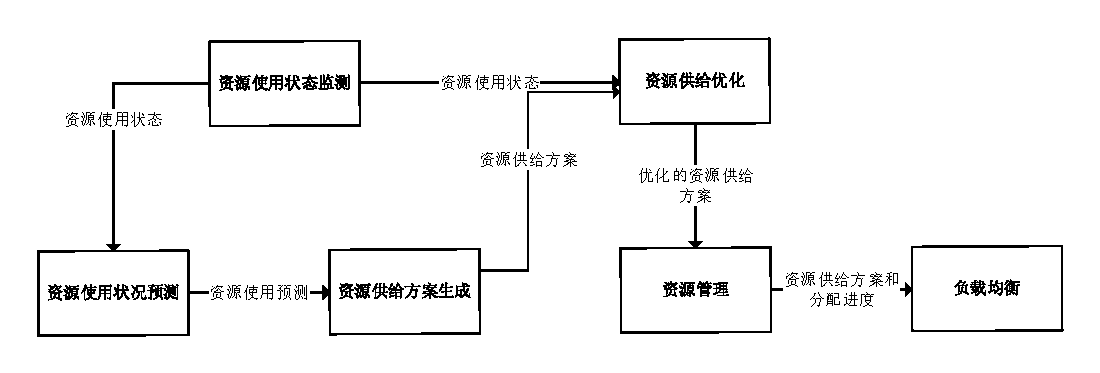
\includegraphics[width=0.9\textwidth]{./figure/sys_design}
\bicaption[fig:sys_design]{系统架构设计}{\textbf{系统架构设计}}{Fig}{System Architecture}
\end{figure}


\section{负载预测模块}

\section{资源供给模块}
\subsection{可用性模型}

\subsection{资源供给方案}\label{sec:provision_design}
侧重于基于预测结果设定资源供给策略,避免频繁的迁移或者增删导致的性能抖动

\section{负载应对选择模块}\label{sec:node_selection}

\section{本章小结}
